%% The following is a directive for TeXShop to indicate the main file
%%!TEX root = diss.tex

\chapter{Introduction}
\label{ch:Introduction}

%\section{Introduction}
Incorporating latent variables to explicitly capture aspects of language, such as semantics, has previously been shown to improve \ac{NMT} quality. This includes difficult scenarios in machine translation, such as translating longer sentences better \cite{Zhang2016VNMT, harshil2018GNMT, Su2018VRNMT}, demonstrating robustness to domain mis-match between training and test data \cite{eikema2018AEVNMT}, as well as enabling word level imputation for noisy sentences \cite{harshil2018GNMT}. 

Another utility of \ac{LVNMT} systems is encoding lexical variation. This is achieved by sampling from the latent variables and using beam search to find semantically similar sentences \cite{schulz2018StochasticDecoder, shen2019diverse}. Generating semantically meaningful sentences is a useful property, because research has shown that synthetically generated \textit{bi-text} can improve translation system quality \cite{sennrich2015ImprovingNMT, edunov2018understandigBackTrans}. In machine translation literature, \textit{bi-text} generally refers to paired sentences from a source language and its translation into a target language. Depending on the model formulation, \ac{LVNMT} systems can likely help build even better machine translation systems by generating synthetic bi-text of sufficiently good quality. 

%One approach for this is backtranslation, where synthetic source sentences are produced by translating the target language into the source language with an existing translation system \cite{sennrich2015ImprovingNMT}. \citet{edunov2018understandigBackTrans} showed that by sampling these synthetic translations instead of sampling them via greedy decoding, the training signal can become more robust to test data, or even help adapt translations systems to domains where data is scarce. Systems have even been developed entirely devoid of bi-text using only monolingual data via backtranslation \cite{lample2018PhraseNeuralUnsuperviseMT, Lample2017UnsuperviseMT, artetxe2017UnsupervisedNMT}, where a system is iteratively improved in an unsupervised fashion. It remains an open area of research to see the impact latent variables models in these contexts.

To our knowledge, much of the research in \ac{LVNMT} applies amortised variational inference to learn the posterior distribution of paired language data. Authors generally have focused on creating variational auto-encoder type models which optimize the evidence lower bound (ELBO) \cite{ kingma2014autoencodingVB, rezende2014stochasticBackprop}. In the context of translation, this involves maximizing the log-likelihood of the conditional distribution $p(\textbf{y} | \textbf{x}, \textbf{z})$ where $\textbf{y}$ is the target language, $\textbf{x}$ is the source language, and $\textbf{z}$ is the introduced latent variable. Authors have assumed the variational posterior distribution is an isotropic Gaussian and learn a variational distribution $q_{\phi}(\textbf{z}\cond{\cdot})$ conditioned on different combinations of available paired sentences.\footnote{ Some condition on both the target and source sentence \cite{Zhang2016VNMT,eikema2018AEVNMT,harshil2018GNMT},  just the target sentences \cite{schulz2018StochasticDecoder}, or even just the source \cite{eikema2018AEVNMT}.} 

%A commonly cited problem in the literature is mode collapse, where the introduced variational distribution $q_{\phi}(z)$ matches the prior distribution and provides uninformative codes \cite{bowman2015GeneratingSent, chen2016VariationalLossyAE, schulz2018StochasticDecoder}. 

The primary focus of this work is to investigate the choice of variational distribution to encode information about translation data. A criticism of variational inference is the limited guarantees on approximating, even asymptotically, the true posterior distribution. There are several empirical findings which suggest that choosing the isotropic Gaussian as the variational distribution family may not truly represent latent aspects of language. One simple example is the power-law distribution behaviour that words exhibit in large corpora of text \cite{koehnSMT2010}. Previous work in language models showed experimental results demonstrating multi-modal distributive behavior even at the character level \cite{ziegler2019LatentNFforDiscrete}. These results suggest that assuming the latent factors follow an isotropic Gaussian distribution is not representative of the true distributive behavior of languages. If latent variables are to be more effectively utilized for machine translation, one needs to consider more flexible variational distributions. 
%one needs to consider more flexible variational distributions to better capture these latent factors of language that the currently de-facto choice of the isotropic Gaussian distribution does not allow.

Normalizing flows represent one variational inference approach towards producing more accurate posterior distribution estimates. They accomplish this by transforming a base distribution into a more complex, possibly multi-modal, distribution \cite{tabak2010densityestimationdual,tabak2013familyofnonparametricdensity}. This change of variables is achieved by invertible functions to transform samples from a chosen base distribution \cite{rezende2015VIwithNF}. This variational approach has the added benefit of empirical findings showing more accurate approximations of target posterior distributions when such distributions are known \cite{rezende2015VIwithNF}.

In the literature, normalizing flows work has seen a number of successes in computer vision, and more recently in natural language processing. Particularly with the task of image generation, normalizing flows have been successful in producing high resolution images \cite{ kingma2016IAF, tomczak2016Householder,kingma2018GLOW, Berg2018SylvesterNF}. \citet{schulz2018StochasticDecoder} proposed normalizing flows as a potential improvement to their work in \ac{LVNMT} systems, but to our knowledge never actually expanded to this direction. Recent works have also considered flows on discrete distributions with modulus operations \cite{hoogeboom2019IntegerDiscreteFlows, tran2019discreteflows}. Continuous normalizing flows have been used for nonautoregressive language modelling as one means to produce meaningful sentences with faster decoding \cite{ziegler2019LatentNFforDiscrete}. Most closely related to our work is the work of \citet{flowseq2019Xuezhe} who created a  non-autoregressive normalizing flow machine translation system.  Our work differs from \citet{flowseq2019Xuezhe} as we consider incorporating normalizing flows with variations of existing autoregressive \ac{LVNMT} systems. 


\begin{figure}[ht]

	\vskip 0.2in
	\begin{center}
		%\textbf{Planar Flows}\par %\midskip
		\centerline{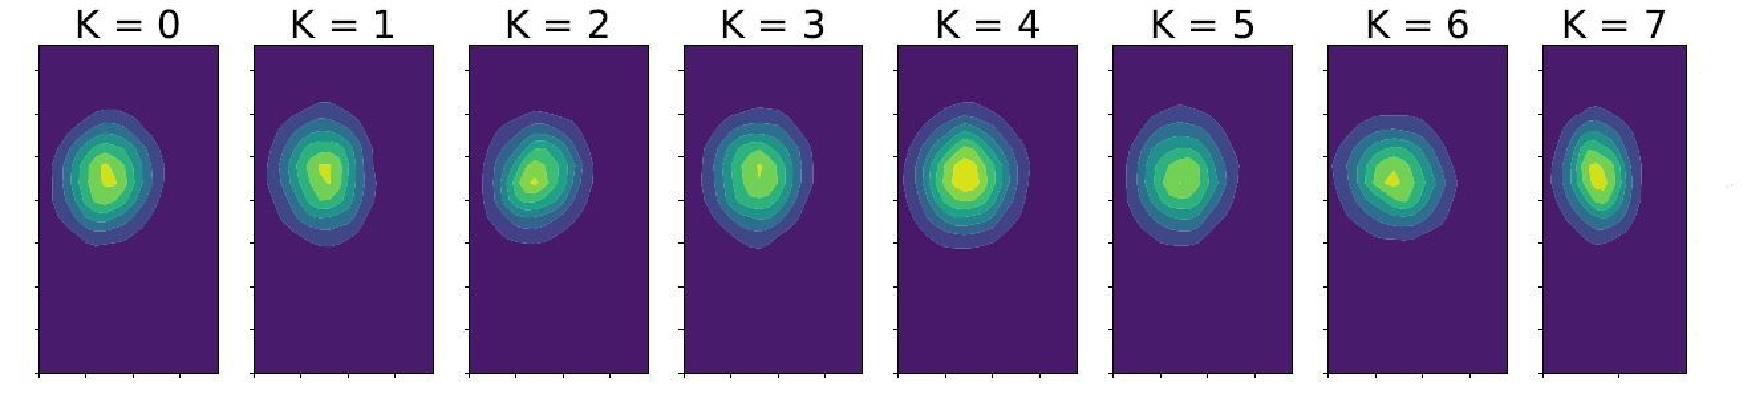
\includegraphics[width=\columnwidth]{planar_flows_plot_edited.pdf}}
		%\textbf{Inverse Autoregressive Flows}\par %\midskip
		\centerline{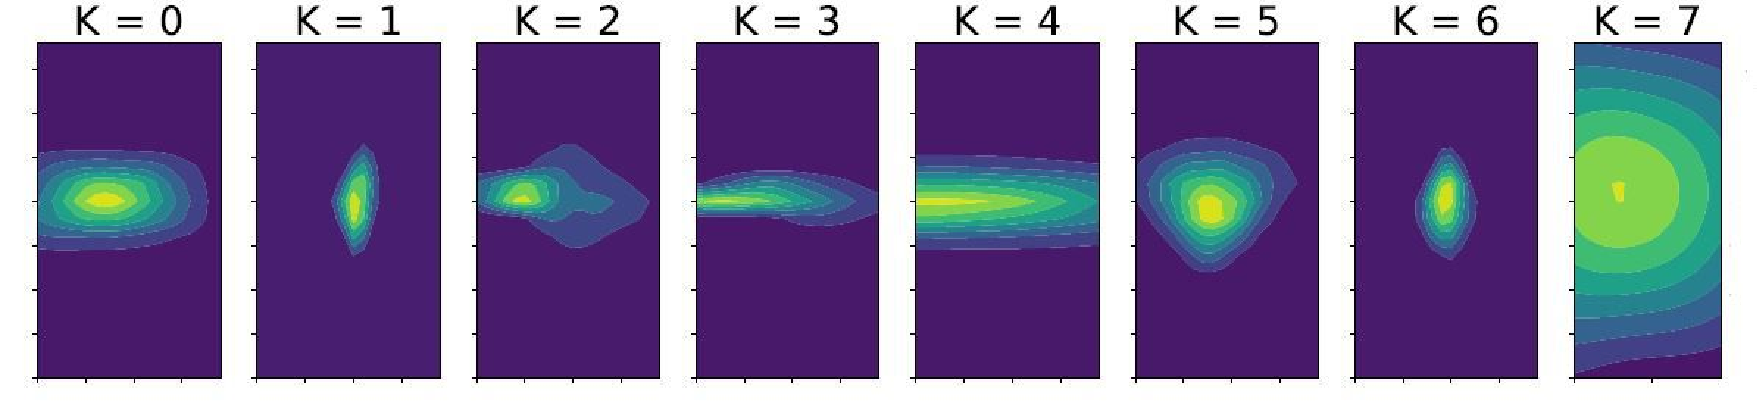
\includegraphics[width=\columnwidth]{iaf_flows_plot_edited.pdf}}
		\caption{Kernel density estimate contour plots of 10,000 samples from $q(z \cond{x, y})$ for each intermittent normalizing flow transformation of the distribution using planar (top) and \ac{IAF} (bottom) flows. The sentence pair is ``Als ich in meinen 20ern war, hatte ich meine erste Psychotherapie-Patientin." (De), translated to ``When I was in my 20s, I saw my very first psychotherapy client." (En)}
	\label{fig:flowsplot}
	\end{center}
	\vskip -0.2in
	\vspace{-4mm}
\end{figure}

We conjecture that normalizing flows are capable of helping achieve better posterior approximations of language factors, and that these improved estimates can help the expressiveness of latent codes in machine translation. Figure~\ref{fig:flowsplot} shows kernel density estimate contour plots of samples after applying normalizing flow transformation
of our distribution, as we further explain in Chapter 6 of this thesis.

%One reason for this is because of the  by introducing an additional expectation dependent on the determinant of the Jacobian of these functions, which hypothesize can allow translation systems to become more robust to a mismatch of domain.   
%As the distribution sampled from will be more complex, this 
%Another motivation for applying normalizing flows to neural machine translation is introducing additional regularization to the ELBO objective.  Some tricks to address this include KL-annealing as well as word dropout to weaken the decoder and force it to rely on the latent variable \cite{bowman2015GeneratingSent}. By incorporating normalizing flows into the objective, we hypothesize the additional regularization provided by these flows will additionally help the models from over-fitting and help prevent the latent variable from being ignored, which particularly can be useful for out-of-domain translation. 

%One other aspect much of literature has ignored is how to produce a global representation of sentences for the latent variable. The general trend has been using a mean-pooling operation over the encoder hidden states before passing the values to non-linear layer operations to produce samples from the amortized inference network \cite{Zhang2016VNMT, Su2018VRNMT, harshil2018GNMT,eikema2018AEVNMT}. We hypothesize this gives unfair weight to words-in-context that may not be as informative to capturing the meaning of sentences. As an example, consider the following two sentences: "I am happy that the dog is healthy" and "I happy dog healthy". Despite the latter being less syntatically structured, the reader would likely infer that both communicate the same underlying semantic concern for an animals well being. To investigate this in the latent variable translation setting, we apply self-attention mechanisms to the encoded states to produce weighted sums of the hidden states to determine whether this intuition is warranted or not.

Overall, we make the following contributions:
\begin{enumerate}
	\item We investigate the use of normalizing flows in \ac{LVNMT} and discuss related considerations and challenges.
	
	\item Our experiments seem to suggest that performance improvements due to the introduction of normalizing flows are minute compared to baseline models. 
	
	\item We find experimentally that when systems are trained with latent variables included, their direct contributions to final performance can be quite small. 
\end{enumerate}

%The rest of this paper is organized as follows.
%In section 2 we discuss related research. In section 3, we review previous works in latent variable machine translation and, as part of our work, we implement one such approach as a probabilistic program. For details on probabilistic programming refer to \citet{janwillem2018IntrotoProbProg}.\footnote{We do not discuss probabilistic programming in this paper, because our work is an application of such languages instead of contributions towards improving probabilistic programming.} In section 4, we discuss incorporating normalizing flows into latent variable machine translations systems and the challenges including normalizing flows. Section 5 discusses our experimental results, and we conclude in section 6. 


